\chapter{Modelling}
\section{Introduction}
In these paragraph we describe how we modeled the Celluar Network described in the specifications.
\begin{itemize}
   \item \textbf{A Web Server}, which generates data in the form of packets to be trasmitted to users. For our pourposes we have defined the class \texttt{UserPackets} which includes a \texttt{start\_time} field and its interface (named \texttt{UserPacket\_m}) includes a getter/setter method to update this field.
   
   The size of each packet is an integer RV \(\sim U(3,75)\), since the service demand has to be uniform and consistent with the frame size. Moreover the packet interarrival time to the antenna has to be an exponential RV, so each packet is generated properly to satisfy this requirements.

   \item \textbf{An Antenna}, which has FIFO queue for each user. Packets received form \textbf{Web Servers} are stored inside queues and then are sent in a unicast way according to the Round Robin policy (which is described in the next section). 
   
   \item \textbf{A Mobile Station}, which personifies a generic user connected to the antenna. On each timeslot it sends a channel quality indicator (CQI), which is a number between 1 and 15 that define the number of bytes the antenna can pack into a Resource Block (RB).
   
   CQIs are integer RVs generated according the following scenarios:
   
   \begin{enumerate} 
    \item Uniform, each user generates a RV \(\sim U(1,15)\)
    \item Binomial, each user generates a RV \(\sim Bin(n,p_i)\), where \(n\) is the number of users, and \( 0<p_i<1\) depends on the user i.
    \end{enumerate} 
\end{itemize}
To build our model and to run rimulations we used the framework \textbf{OMNeT++ v5}, so each item described before is defined by a \texttt{*.ned} file.
Each \texttt{Mobile Station} computes some statistics: slotted throughput (related to each time slot) and response time of received packets. The \texttt{Antenna} compute also statistics about the frame filling, which we will describe later.

The \texttt{CellularNetwork.ned} file shows how the previous modules are connected to obtain the network. Since frames are sent in a unicast way, there are multiple instances of the Web Server module, one for each Mobile Station, seeded in a different way in order to have IID RV.

The obtained network, by setting \(n=10\), is the following: 
\begin{figure}[H]
  \centering
  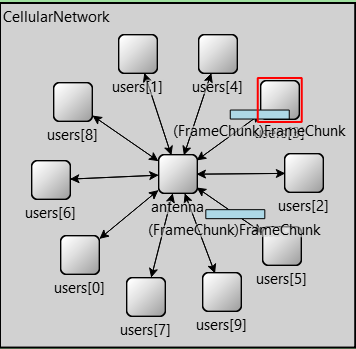
\includegraphics{images/network_simulations}
  \caption{Simulated Network (omnet++)}
  \label{fig:simulated_network}
\end{figure}

\section{Frame Chunks}
  Packets are delivered to users by enveloping that inside RBs. As requested by specifications \(RBsize\textsubscript{i,t\textsubscript{j}}=f(CQI\textsubscript{i,t\textsubscript{j}})\) where \(i\) is index of \textit{user}, and \(t\textsubscript{j}\) is index of \textit{timeslot}.
  To do that, the scheduler receives CQIs from the \texttt{Mobile Stations} at beginnig of each time slot, then compute every \(RBsize\textsubscript{i,t\textsubscript{j}}\) and fills the frame according to scheduling policy. Note that a frame can carry RBs for different users so, generally speaking, a frame in a specific time slot \(t\textsubscript{j}\) can have RBs of different size. To cope these requirements we defined a new module \texttt{Frame Chunk} wich groups all RBs addressed to a specific \texttt{Mobile Station}. By introducing this module we can consider a frame as a collection of \texttt{Frame Chunks}. To deliver the whole frame we must send each \texttt{Frame Chunk} to its user in a unicast way.

\section{Schedulers}
  In this section we will analyze the frame filling policy wich are defined in the module \texttt{Scheduler}.
  Let's consider a user \(0\leq i < n\). Starting from user \(i\), the scheduler allocates a new \texttt{Frame Chunk} and fills it with packets taken from the \texttt{FIFOQueue\textsubscript{i}}. A \texttt{Frame Chunk} is considered full if it contains 25 RBs because it corresponds to the whole frame. At the next time slot will be served the user \((i+1)\textnormal{mod }n\). If the frame is not full the scheduler must allocate others \texttt{Frame Chunks} in order to fill the residual space using one of the two following policies. 

\begin{itemize}
%\subsection{Round-Robin Frame Fill}
  \item \textbf{Round-Robin Frame Fill}
  The residual space  in the frame is filled by considering the following \texttt{FIFOQueues\textsubscript{j}} \(j \in \{ (i+1)\textnormal{mod } n,(i+2)\textnormal{mod }n,\ldots \} \)
%\subsection{Best CQI based Frame Fill}
  \item \textbf{Best CQI based Frame Fill}
   The residual space in the frame is filled by considering the users with the best(highest) CQI in a decreasing order. In the case of \(CQI\textsubscript{i}=CQI\textsubscript{j} \mid i < j\) is selected the user \(i\).
\end{itemize}
We will analyze the effect of both policy to performace regarding the throughput and the response time for each user with varying workloads.

\section{Constants}
In the following chapters, if not different specified, we will consider this constants.
\begin{itemize}
\item \textbf{Number of resource block}, \(\#RB = 25\)
\item \textbf{Number of users}, \(n = 10\)
\item \textbf{Max RB size}, \(RBsize\textsubscript{max} = 93\)
\item \textbf{Max packet size}, \(packetsize\textsubscript{max} = 75\)
\item \textbf{Timeslot period}, \(T\textsubscript{slot} = 1\textnormal{ms}\)
\end{itemize}